% !TeX root = ../main.tex

In this section, the reader will be provided with a comprehensive presentation of the results derived from our experiments. These results are juxtaposed not only amongst themselves but also with results from foundational studies, such as the base paper~\cite{zhuang2022randomness}, to highlight differences and commonalities.\\

Throughout this results section, accompanying each set of findings will be explanatory text. This narrative is designed to guide readers, helping them navigate through the figures and understand the salient points. While interpretations and deeper discussions on implications will be reserved for subsequent sections, this portion is instrumental in building a foundational understanding of our experimental outcomes.


\section{Aggregated Results}

In this section, we illuminate the comprehensive performance metrics across diverse configurations and datasets. For contextual clarity, we juxtapose our findings with established results from extant literature. The primary objective of providing these metrics was to offer readers a foundational understanding of the experimental landscape and the inherent complexities involved.\\

It is imperative to underscore that our investigations did not prioritize achieving state-of-the-art outcomes. Instead, our primary objective centers around exploring the underlying randomness inherent in the models. Therefore, our resource allocation primarily emphasized this investigation over optimizing performance benchmarks.\\

For each experiment, we adopt conventional baselines, ensuring minimal modifications in terms of performance enhancement. Our methodologies mainly deviate from these baselines in the realm of experimental design and the integration of reproducibility protocols. A noteworthy adaptation is our incorporation of an additional optimizer into the pipeline. While the baseline configurations predominantly rely on a singular optimizer, we introduce a secondary one, necessitating minimal adjustments in hyperparameter tuning.
\clearpage
Shifting focus to the CIFAR-10 dataset, Table \ref{tab:cifar10_updated} delineates the accuracy scores we achieved across various seeds and optimizers. Deterministic columns shows the mean of the five runs for that spefific configuration. We also present the difference between that mean and non-deterministic run in percentage. Owing to the equitably distributed classes in the CIFAR-10 dataset, accuracy remains the predominant metric within the research community.\\

Upon examination of the results, there's a discernible trend where the SGD optimizer consistently outperforms the ADAM optimizer in terms of accuracy, regardless of the seed. Specifically, the highest accuracy we observe with SGD is approximately 94.81\% with a seed value of 42 in the deterministic setting. In contrast, ADAM's performance peaks around 93.07\% with a seed value of 180698 in the non-deterministic mode.\\

This differential further underscores the nuanced behavior of optimizers and their sensitivities to factors like initialization seeds. Notably, our findings resonate with benchmark data from extant literature~\cite{zhuang2022randomness}, affirming the reliability of our evaluations. It should be emphasized that our approach towards CIFAR-10 predictions strictly followed established methodologies, ensuring no employment of advanced techniques.
\begin{table}[h!]
  \centering
  \caption{Results for CIFAR-10 (Accuracy with Difference from Non-deterministic Mean)}
  \label{tab:cifar10_updated}
  \begin{tabularx}{\textwidth}{XlS[round-mode=places, round-precision=2]S[round-mode=places, round-precision=2]S}
  \toprule
     Seed & Optimizer & {Non-deterministic} & {Deterministic} & {Difference from Mean (\%)} \\
  \midrule
    0 & ADAM & 92.662 & 92.19 & -0.509 \\
       & SGD & 94.804 & 94.96 & 0.164 \\
  \midrule
    180698 & ADAM & 93.068 & 92.22 & -0.910 \\
       & SGD & 94.746 & 94.93 & 0.194 \\
  \midrule
    314 & ADAM & 92.178 & 92.17 & -0.009 \\
       & SGD & 94.814 & 94.71 & -0.110 \\
  \midrule
    3407 & ADAM & 92.568 & 92.72 & 0.164 \\
       & SGD & 94.726 & 94.59 & -0.144 \\
  \midrule
    42 & ADAM & 92.536 & 92.71 & 0.188 \\
       & SGD & 94.756 & 94.81 & 0.057 \\
  \bottomrule
  \end{tabularx}
\end{table}

From the data presented in Table \ref{tab:cifar10_updated}, it is evident that the choice of optimizer plays a important role in the observed outcomes. Previous studies in the literature have posited that SGD tends to outperform ADAM when applied to the CIFAR-10 dataset~\cite{gupta2021adam}. Our empirical findings corroborate this assertion. In experiments it is understood that, the ADAM optimizer demonstrates a protracted convergence trajectory, necessitating an increased number of epochs to approach an optimum. Intriguingly, the global optima identified by ADAM diverges from that ascertained by SGD.
In our analysis, when comparing our findings with the results presented in He et al.~\cite{he2016identity}, which employed a more extensive layer architecture, it is evident that our outcomes are consistent and fall within a similar performance range.\\

    
\begin{table}[h!]
  \centering
  \caption{Results for SDNET (F1-Score with Difference from Non-deterministic Mean)}
  \label{tab:sdnet_updated}
  \begin{tabularx}{\textwidth}{XlSSS}
  \toprule
     Seed & Optimizer & {Non-deterministic} & {Deterministic} & {Difference from Mean (\%)} \\
  \midrule
    0 & ADAM & 0.9328 & 0.9370 & 0.449 \\
       & SGD & 0.9249 & 0.9264 & 0.162 \\
  \midrule
    180698 & ADAM & 0.9345 & 0.9382 & 0.395 \\
       & SGD & 0.9233 & 0.9212 & -0.227 \\
  \midrule
    314 & ADAM & 0.9323 & 0.9314 & -0.096 \\
       & SGD & 0.9242 & 0.9158 & -0.909 \\
  \midrule
    3407 & ADAM & 0.9347 & 0.9329 & -0.192 \\
       & SGD & 0.9185 & 0.9203 & 0.196 \\
  \midrule
    42 & ADAM & 0.9322 & 0.9337 & 0.161 \\
       & SGD & 0.9264 & 0.9231 & -0.356 \\
  \bottomrule
  \end{tabularx} 
\end{table}

    
    
For detecting concrete cracks, we use the F1-score as our main metric, and the outcomes are shown in Table \ref{tab:sdnet_updated}. We notice differences in performance based on the optimizer used. However, it's not clear-cut which optimizer is better, and that's not our main focus anyway. Additionally, just like with the CIFAR-10 data, our results for concrete crack detection which is achieved by a light model are sufficient for real-world situations. 
Furthermore, our results demonstrate improved performance compared to the foundational paper associated with the dataset~\cite{dorafshan2018sdnet2018}, attributable to our selection of more recent and superior model.
% For example, Meng et. al.~\cite{meng2023real} talk about using a model on a drone to spot cracks in real time.
% Our results can be compared with those from (source).\\
\\
\\
\\
\begin{table}[h!]
  \centering
  \caption{Results for CBIS-DDSM (AUC-Score with Difference from Mean)}
  \label{tab:cbis-ddsm_updated}
  \begin{tabularx}{\textwidth}{XlS[round-mode=places, round-precision=4]S[round-mode=places, round-precision=4]S[round-mode=places, round-precision=4]}
  \toprule
     Seed & Optimizer & {Non-deterministic} & {Deterministic} & {Difference from Mean (\%)} \\
  \midrule
    0 & ADAM & 0.7926 & 0.7817 & -1.376 \\
       & SGD & 0.7669 & 0.7735 & 0.859 \\
  \midrule
    180698 & ADAM & 0.7814 & 0.7716 & -1.257 \\
       & SGD & 0.7642 & 0.7773 & 1.714 \\
  \midrule
    314 & ADAM & 0.7775 & 0.7936 & 2.073 \\
       & SGD & 0.7718 & 0.7770 & 0.674 \\
  \midrule
    3407 & ADAM & 0.7969 & 0.7877 & -1.152 \\
       & SGD & 0.7723 & 0.7656 & -0.866 \\
  \midrule
    42 & ADAM & 0.7838 & 0.7965 & 1.619 \\
       & SGD & 0.7724 & 0.7695 & -0.376 \\
  \bottomrule
  \end{tabularx}
\end{table}


Table \ref{tab:cbis-ddsm_updated} showcases the AUC scores obtained for the CBIS-DDSM dataset across various seed values and using two distinct optimizers: ADAM and SGD. The AUC (Area Under the Curve) score is a crucial metric in medical imaging as it provides insights into the model's ability to distinguish between positive and negative classes, with a score closer to 1 indicating superior discriminative power.
Our findings align with those presented in the work of~\cite{DBLP:journals/corr/abs-2002-07613}, albeit without employing GMIC (Globally-aware Multiple
Instance Classifier), which is known for its low-memory consumption while enabling higher resolution. From the table, we observe a close competition between the ADAM and SGD optimizers across different seed values. While certain seeds yield slightly higher AUC scores for the ADAM optimizer in the non-deterministic setting, others favor the SGD optimizer in the deterministic mode.\\

Such variances underscore the significance of random seed initialization in the training process and how it can influence the performance of different optimizers. Furthermore, the results highlight the importance of considering both deterministic and non-deterministic settings in model evaluations, especially in critical applications like medical imaging.\\    

In general, out of a total of 180 runs, the table below summarizes the worst, average, and best performance metrics obtained across the three tasks at hand.

\begin{table}[htbp]
  \centering
  \caption{Summary of Performance Metrics}
  \label{tab:performance_summary}
  \begin{tabular}{lccccc}
      \toprule
      Dataset & Metric & Minimum Value & Mean Value & Maximum Value  \\
      \midrule
      CIFAR-10 & Accuracy (\%) & 91.5 & 93.9 & 95.1  \\
      CBIS-DDSM & AUC Score & 0.750 & 0.775 & 0.805  \\
      SDNET & F1-Score & 0.912 & 0.928 & 0.938 \\
      \bottomrule
  \end{tabular}
  \vspace{1em}  % adds some space between the table and the legend
  \begin{minipage}{\textwidth}
    \small
    Note: The metrics presented do not differentiate between the optimizers used. 
  \end{minipage}
\end{table}

Best values in CIFAR-10 and CBIS-DDSM are from non-deterministic runs, indicating a beneficial impact of randomness. Conversely, in SDNET, the highest F1-Score is achieved with a fixed seed of 180698. However, the minimum performance metrics were observed in non-deterministic runs, suggesting that these instances were adversely impacted by the inherent randomness.

\section{Variances in Results}

In this section, we present the variances in the results. We calculate the variance by calculating the standard deviation using the 
following formula. 

\begin{equation}
  \sigma = \sqrt{\frac{1}{N} \sum_{i=1}^{N} (x_i - \mu)^2}
  \end{equation}
  
  Where:
  \begin{itemize}
      \item \( \sigma \) represents the standard deviation.
      \item \( N \) denotes the number of observations.
      \item \( x_i \) signifies each individual observation.
      \item \( \mu \) is the mean of the observations.
  \end{itemize}

Calculating the standart deviation informs us that how much the results deviate from the mean. Higher 
standart deviation indicates that the reproducibility is less and thus the credibility of the results are endangered. It is important here to note that
higher number of samples used in the standart deviation calculation can help better estimate the variances and covers all the possible extremum values thus increases scientific validity. 
Due to limitations, we use five identical runs to calculate the standart deviation. We can look at the variances
in performance metrics, weights and runtimes. Each could give us the different aspects and affects of the reprodubility on deep learning tasks. We present the results of the weight analysis in the next section.


\subsection{Performance Variance}

For each task, distinct pipelines and performance metrics are employed, rendering direct performance comparisons infeasible. Nonetheless, by comparing the variances, we can infer the sensitivities of these tasks to inherent randomness. The subsequent discussion presents the variances in performance metrics across three distinct tasks.

\begin{figure}[h!]
      \centering
      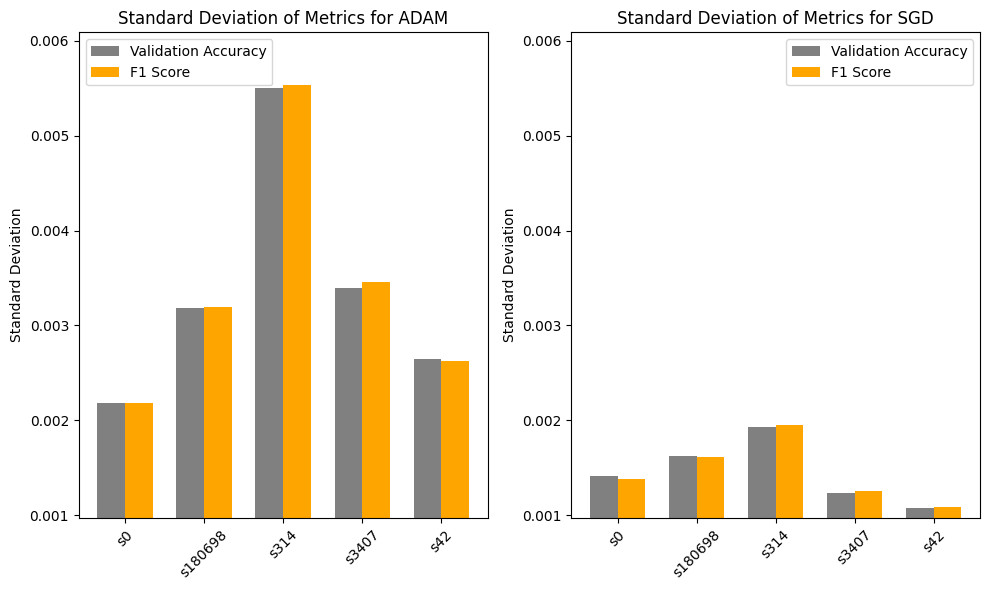
\includegraphics[width=0.8\textwidth]{figures/cifar_std_results.png}
      \caption{Standard Deviation of Performance Metrics for CIFAR-10}
      \label{fig:cifar10_var}
\end{figure}

Referring to Figure \ref{fig:cifar10_var}, the CIFAR-10 task showcases variances in both the F1-Score and Accuracy metrics across two different optimizers. Distinct seed configurations yield varying variance values. A notably higher variance is observed with the ADAM optimizer, suggesting that this optimizer might exhibit greater sensitivity to initial conditions or inherent randomness. The variance values span a range between 0.001 and 0.006, with the peak variance observed for the configuration using seed 314, approximating 0.0055. A close examination of the data also reveals negligible differences in variance between the F1-Score and Accuracy metrics, indicating their congruence in this context.\\


\begin{figure}[h!]
  \centering
  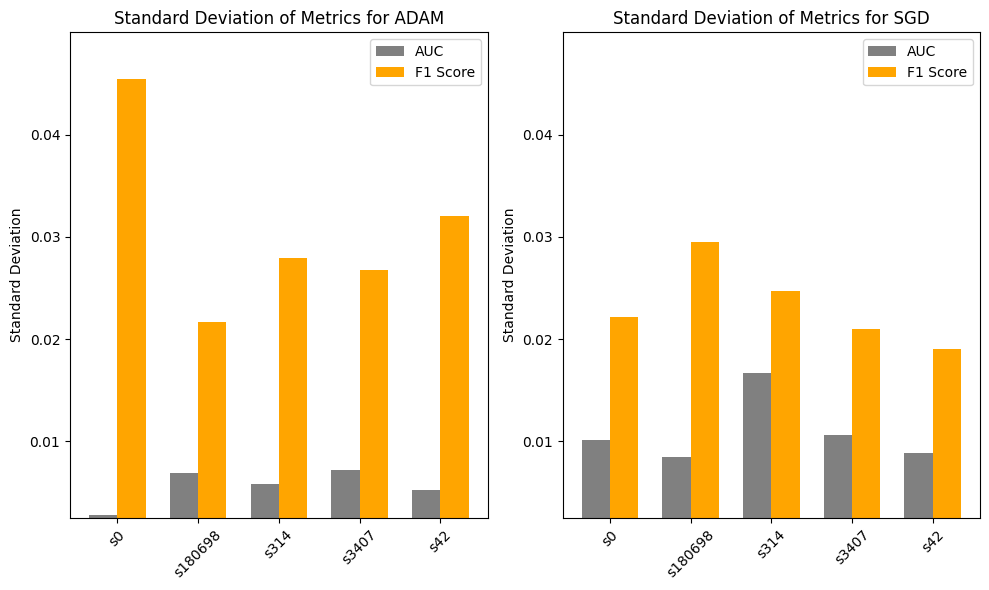
\includegraphics[width=0.8\textwidth]{figures/mammo_results_std.png}
  \caption{Standard Deviation of Performance Metrics for CBIS-DDSM}
  \label{fig:cbisddsm_var}
\end{figure}

Figure \ref{fig:cbisddsm_var} illustrates the standard deviation values for the CBIS-DDSM task. The SGD optimizer exhibits pronounced variances in the AUC score, whereas the ADAM optimizer demonstrates heightened variances in the F1-score. Notably, the overall variance in the F1-score surpasses that of the AUC scores. Moreover the stability of the SGD optimizer against variance appears more consistent, given the relatively minor differences in variances between performance metrics compared to the ADAM optimizer. Moreover, the range of standard deviation values is approximately an order of magnitude greater than observed in the CIFAR-10 task, with the maximum value reaching 0.05 and the minimum at 0.009, particularly evident for the ADAM optimizer with seed 0.\\

\begin{figure}[h!]
  \centering
  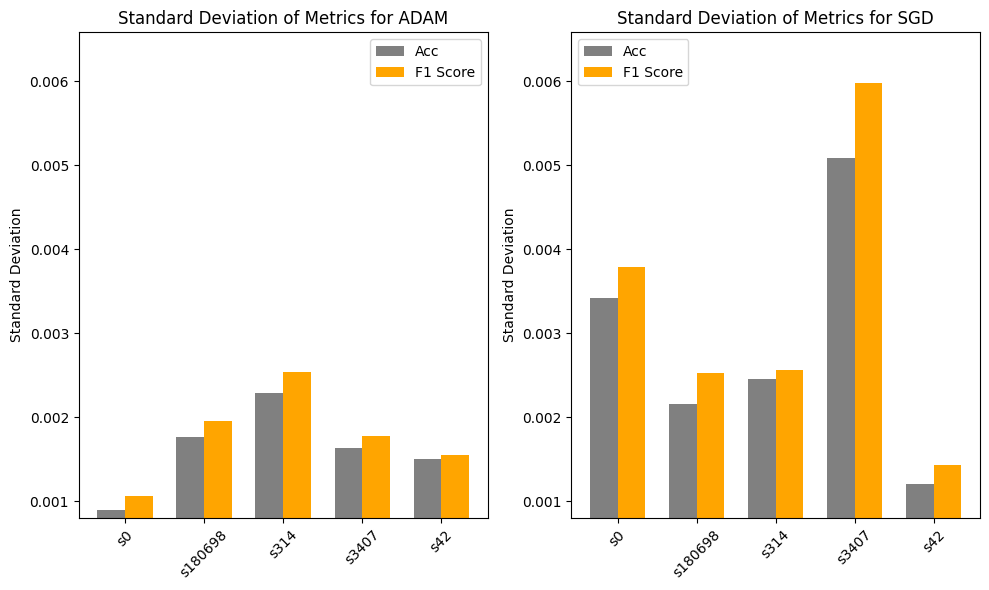
\includegraphics[width=0.8\textwidth]{figures/crack_results_std.png}
  \caption{Standard Deviation of Performance Metrics for SDNET}
  \label{fig:sdnet_var}
\end{figure}

Figure \ref{fig:sdnet_var} presents the variances in performance metrics for the concrete crack detection task. A relatively larger disparity between the F1-score and Accuracy is observed compared to the CIFAR-10 task. Contrary to the previous tasks, the SGD optimizer exhibits higher overall variances for this task. However, the variance range aligns closely with that of the CIFAR-10 task. The apex of variance is identified with seed 3407 using the SGD optimizer.\\

In our analysis of performance variances across tasks, we discerned distinct variability ranges and sensitivities to CUDA-induced randomness. These findings facilitate a deeper understanding of the ramifications of CUDA-related randomness on model performance.\\

\subsection{Runtime and Performance Tradeoff between Deterministic and Non-deterministic Execution}

Since for each seed and optimizer configuration we have one fully deterministic configuration. It would be wise to look at the performances and runtimes to determine the tradeoffs.\\

\begin{figure}[h!]
  \centering
  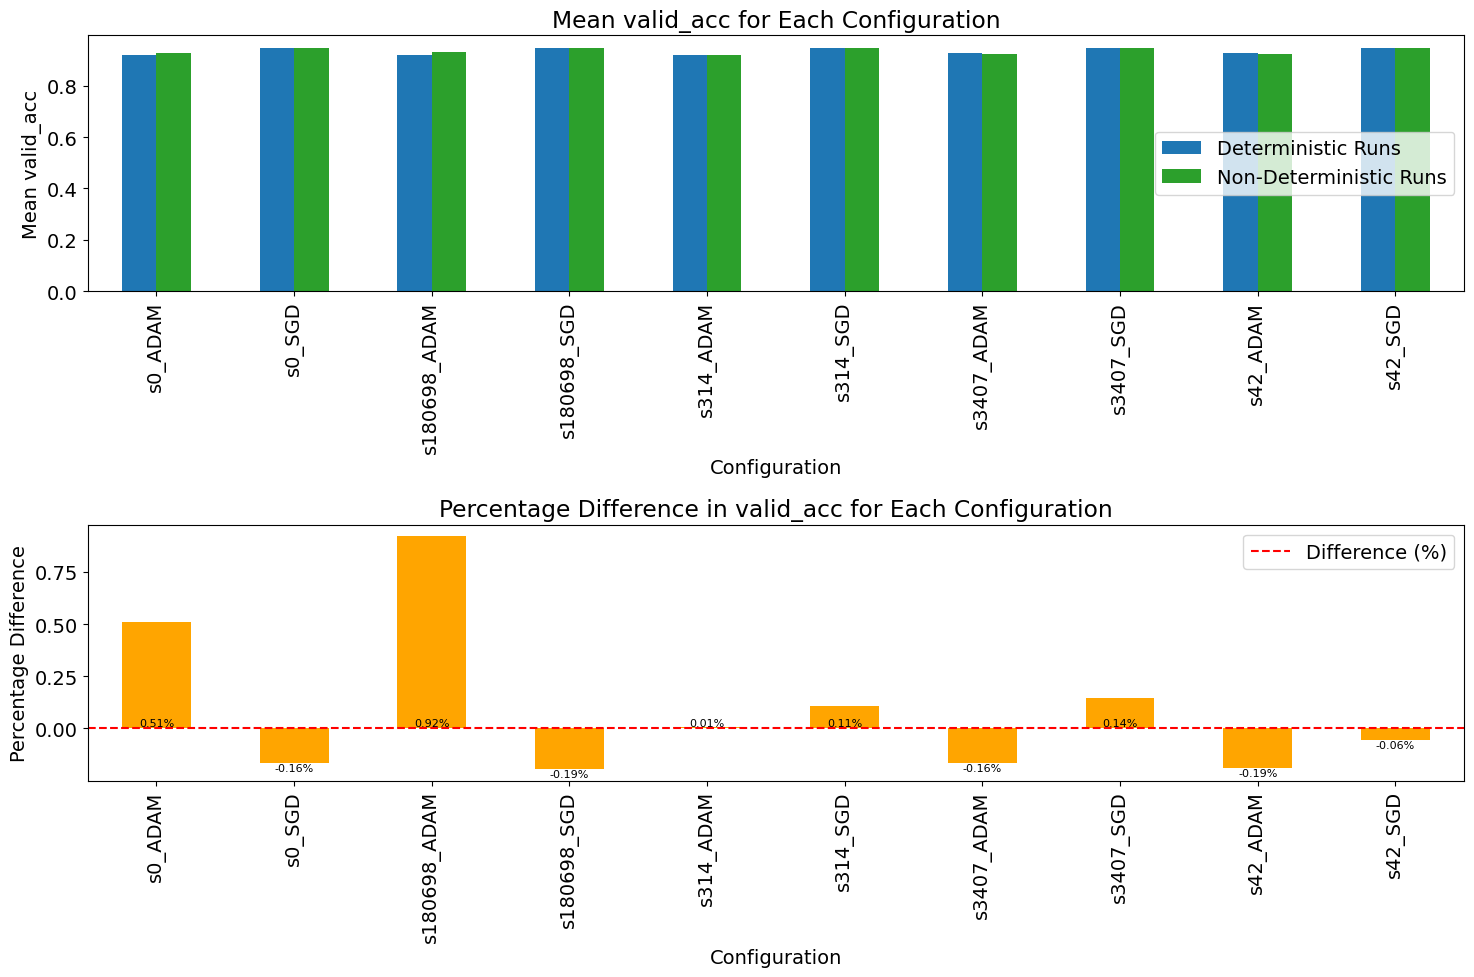
\includegraphics[width=1\textwidth]{figures/cifar_performance.png}
  \caption{CIFAR-10 Differences in Performance between Deterministic and Non-deterministic}
  \label{fig:cifar10_dif_per}
\end{figure}

Above we see the performance difference for CIFAR-10 task, it is clear that at first look there is no jump in performance but on some cases non deterministic execution can benefit from randomness and produce higher results.\\
We observe up to 1\% performance increase in Adam optimizer when using seed value as 180698. From the figures, there is no clear signs that would show that fully deterministic execution increases performance or vice versa.\\

\begin{figure}[h!]
      \centering
      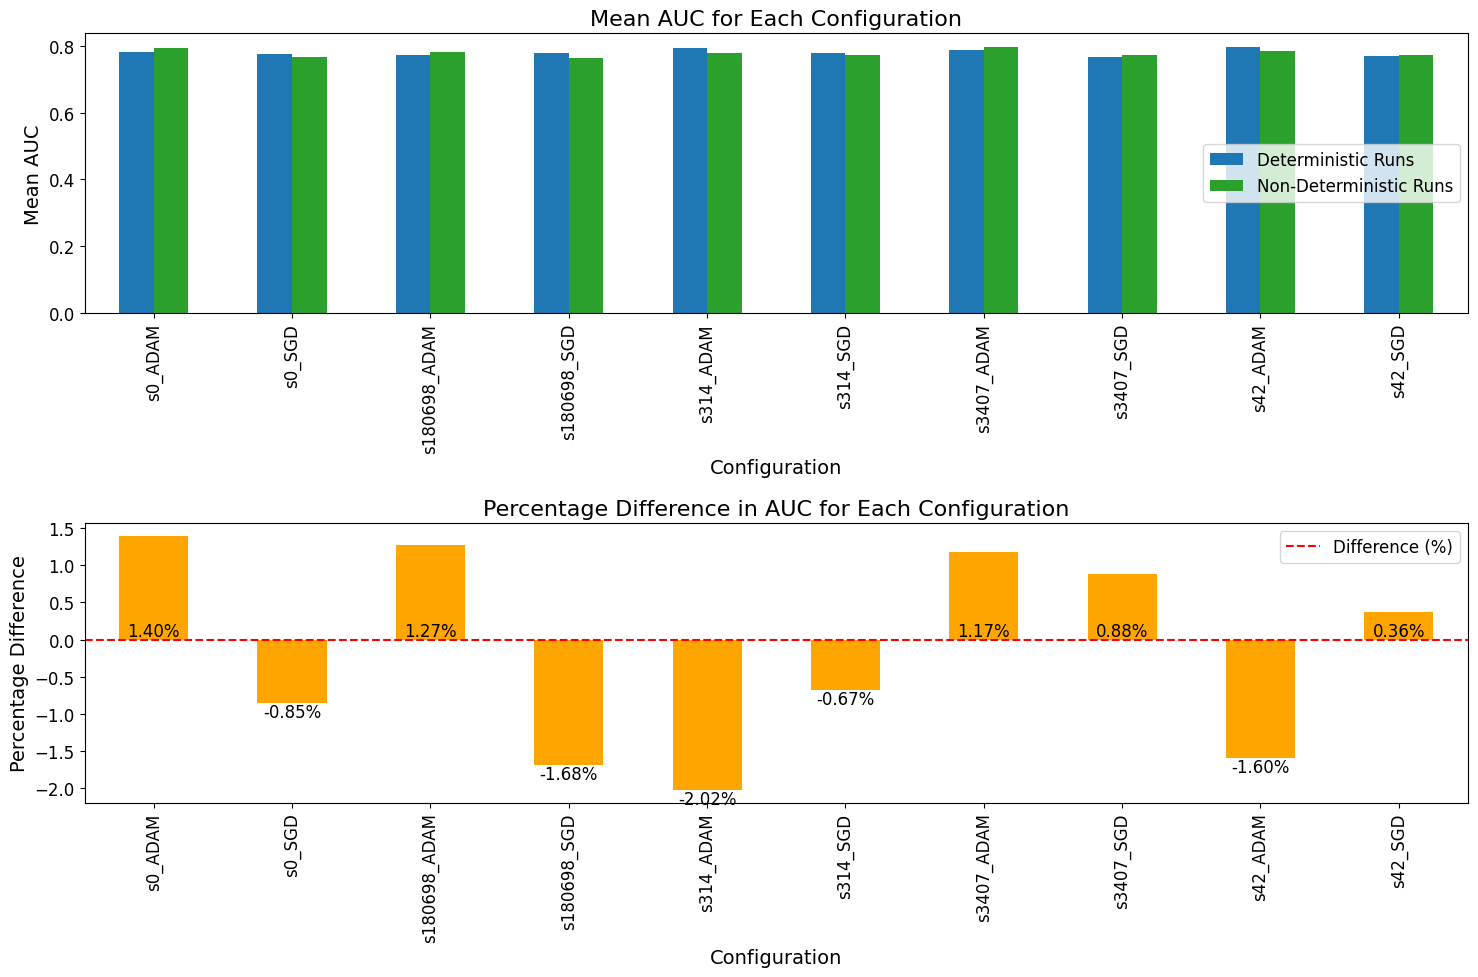
\includegraphics[width=1\textwidth]{figures/mammo_performance.png}
      \caption{CBIS-DDSM Differences in Performance between Deterministic and Non-deterministic}
      \label{fig:cbisddsm_dif_per}
\end{figure}

For the CBIS-DDSM dataset we observe relatively higher differences in AUC scores. There is no clear direction but fully deterministic execution reduced the performance by up to 2 for the seed 314 and increased up to 1.4 for the seed 0.
We observe these extremum values in ADAM optimizer indicating a less stability.\\

\begin{figure}[h!]
      \centering
      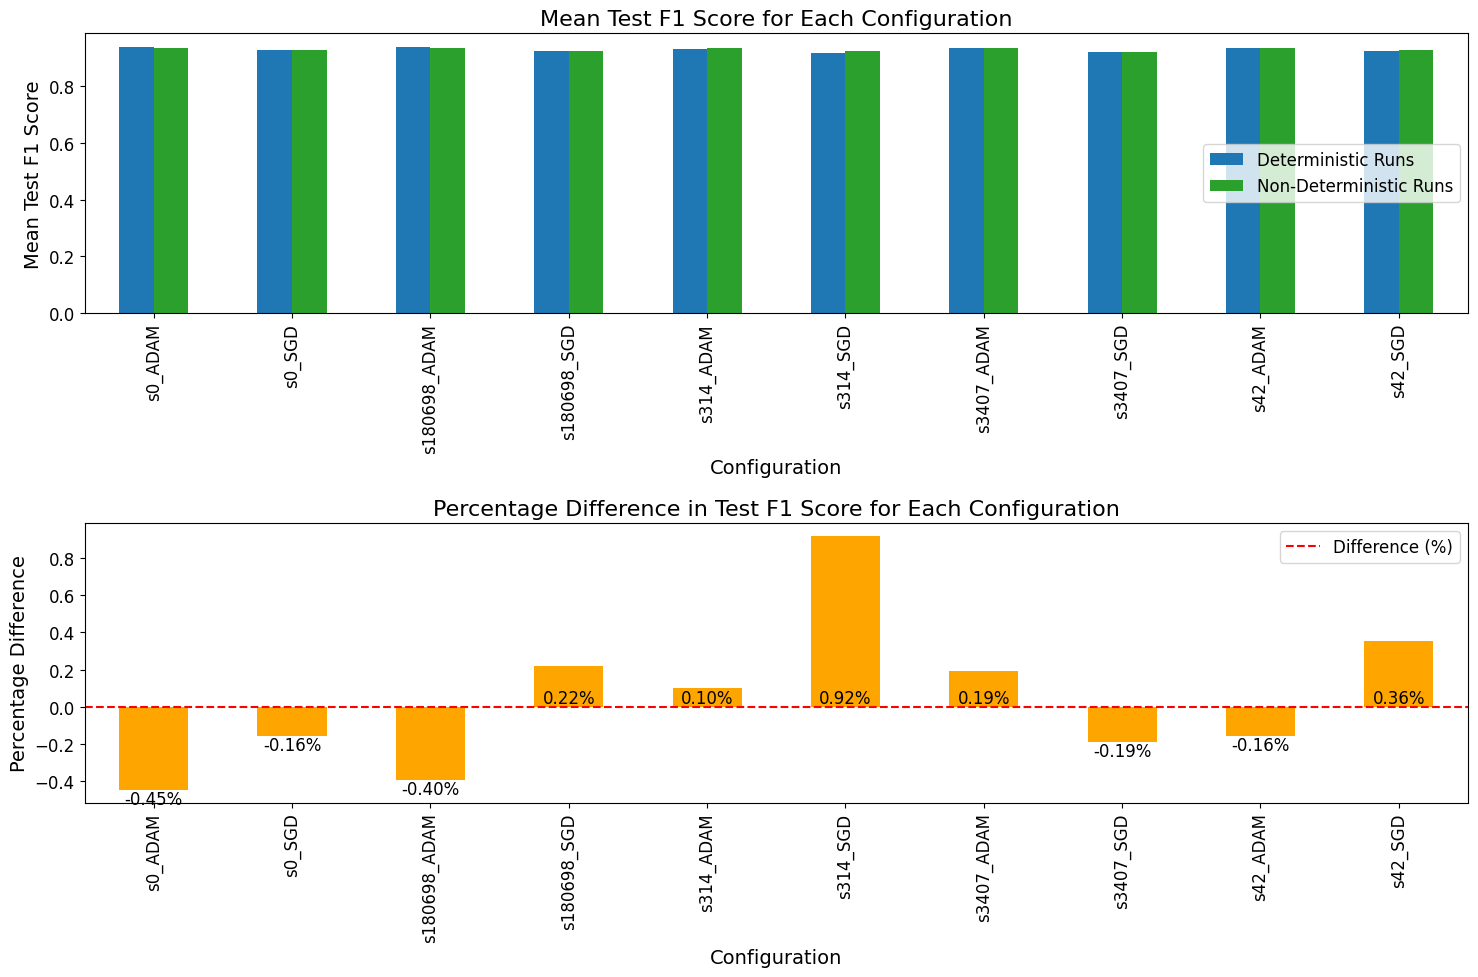
\includegraphics[width=1\textwidth]{figures/crack_performance.png}
      \caption{SDNET Differences in Performance between Deterministic and Non-deterministic}
      \label{fig:sdnet_dif_per}
\end{figure}
In concrete crack detection experiments, like others, we see no visible direction. The range of increase and decrease also similar like CIFAR-10 task. Unlike CIFAR-10, however, highest benefit gained in SGD optimizer with seed as 314. 

\clearpage

\subsection{In Runtime}
\begin{figure}[h!]
      \centering
      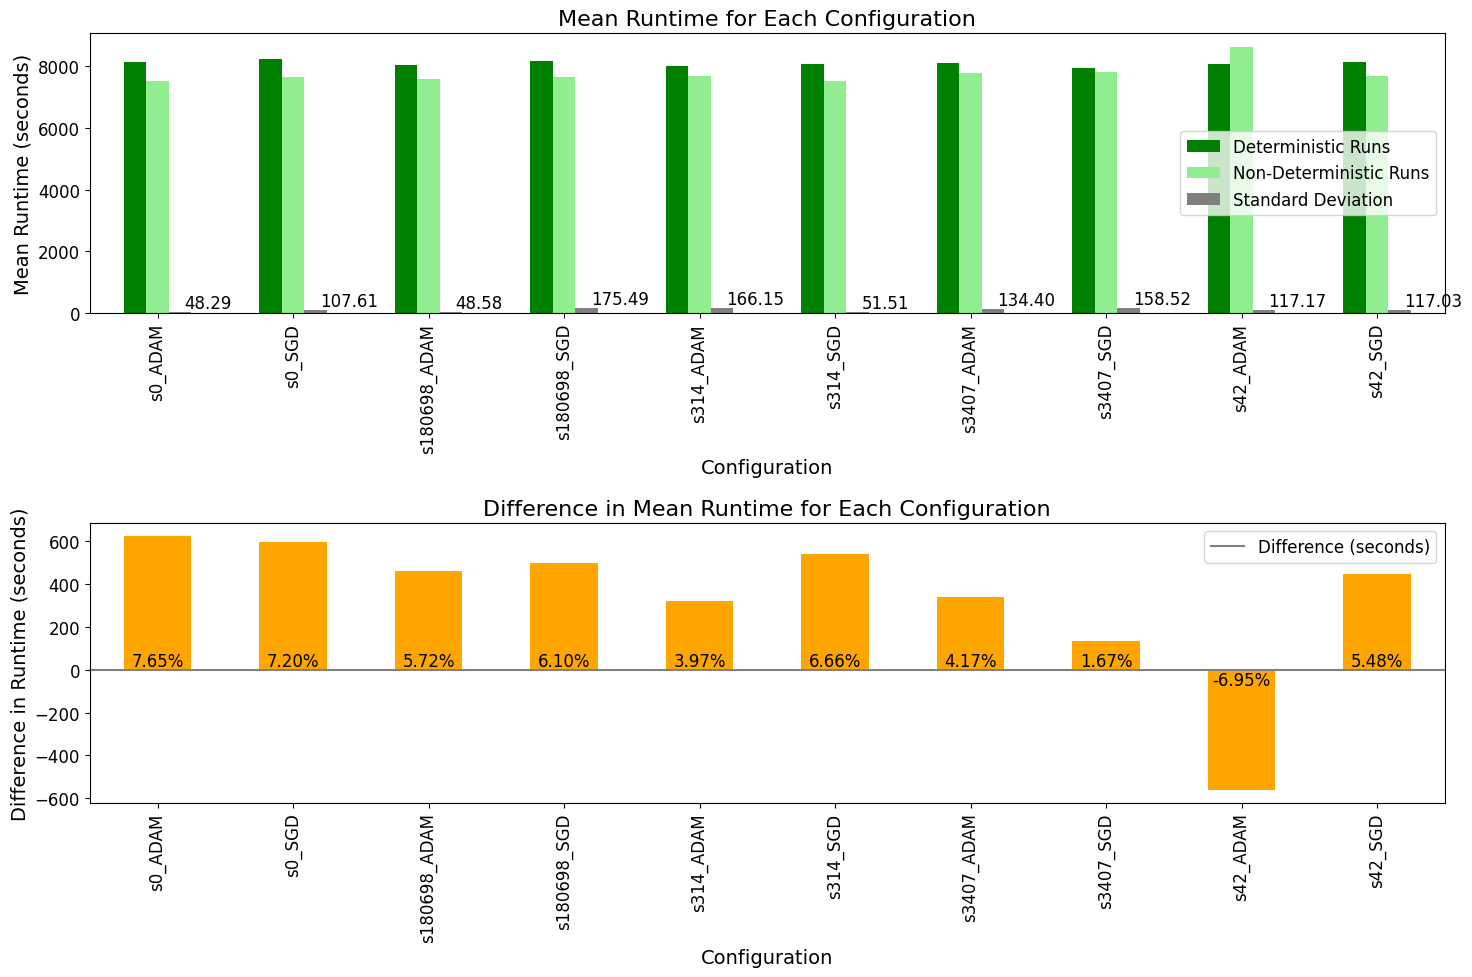
\includegraphics[width=1\textwidth]{figures/cifar_runtime.png}
      \caption[CIFAR-10 Differences in Runtime between Deterministic and Non-\\deterministic]{CIFAR-10 Differences in Runtime between Deterministic and Non-deterministic}
      \label{fig:cifar10_dif_run}
\end{figure}

In runtimes, calculated in seconds, we observe from the figure that deterministic execution takes longer up to 7.65 percent which is in seed value 0 and optimizer as ADAM. 
Note that, longer execution time heavily dependend on the used algorithm change due to deterministic algorithm choices by PyTorch.


\begin{figure}[h!]
    \centering
    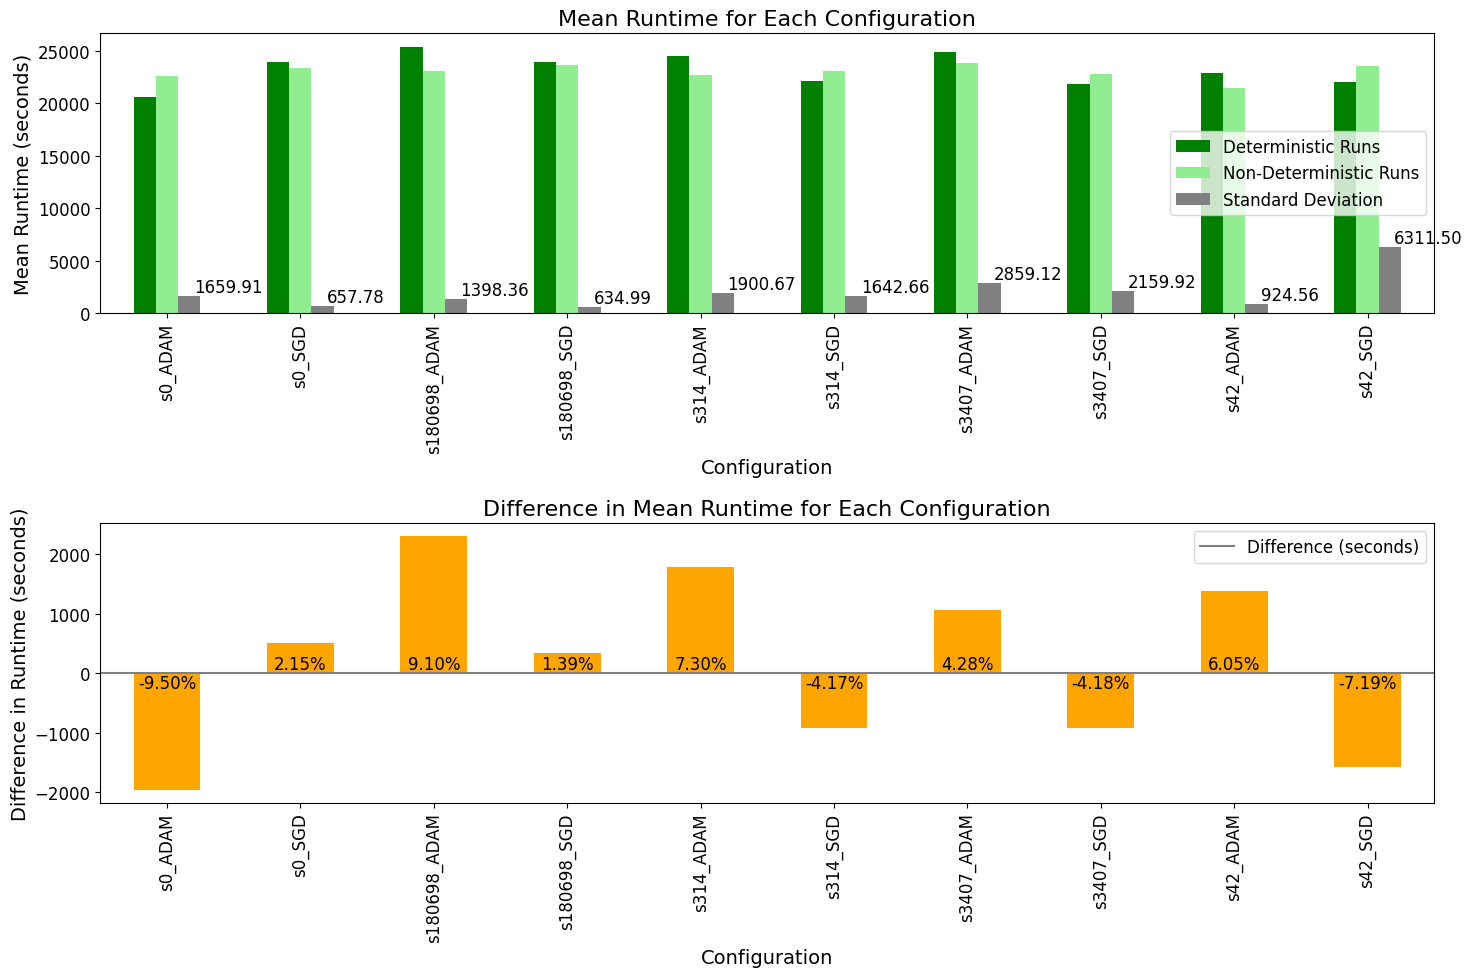
\includegraphics[width=1\textwidth]{figures/mammo_runtime.png}
    \caption{CBIS-DDSM Differences in Runtime between Deterministic and Non-deterministic}
    \label{fig:cbisddsm_dif_run}
\end{figure}

Runtime difference for CBIS-DDSM dataset presented above. Unlike the CIFAR-10, we observe different pattern and no clear direction of runtime tradeoff for the deterministic execution. According the figure, deterministic execution could increase the runtime up to 9 and decrease as well. We observe this extremums in ADAM as seed 0 and ADAM as 180698, respectively. The differences in SGD optimizer are less than the ones in the ADAM. 

\begin{figure}[h!]
    \centering
    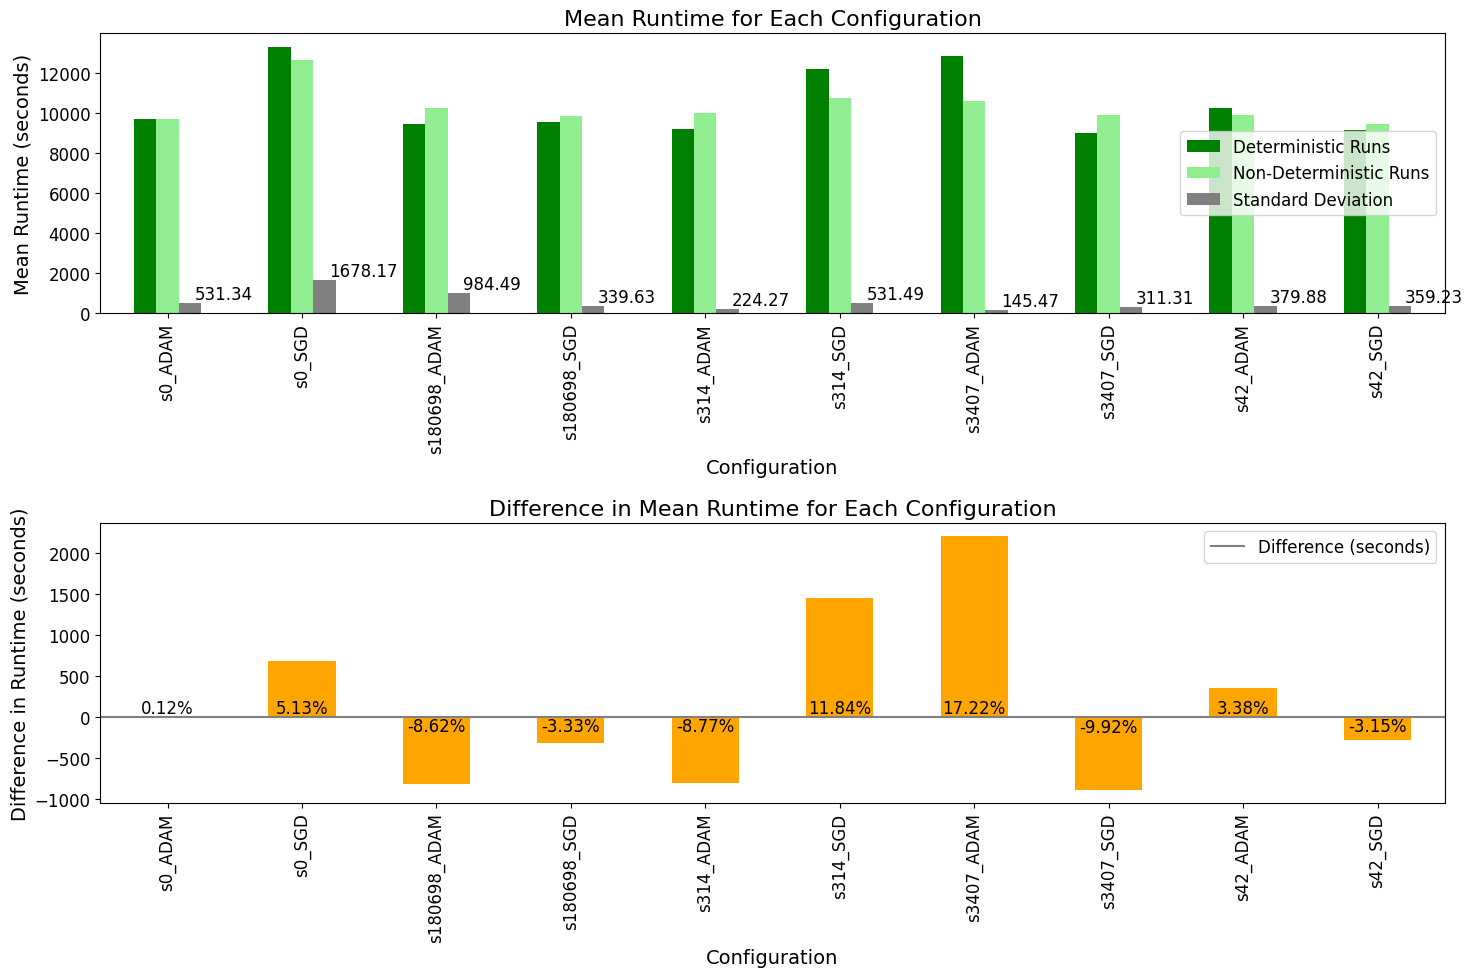
\includegraphics[width=1\textwidth]{figures/crack_runtime.png}
    \caption{SDNET Differences in Runtime between Deterministic and Non-deterministic}
    \label{fig:sdnet_dif_run}
\end{figure}

As for the concrete crack detection, deterministic execution increased the execution time up to 17 in ADAM configuration while second high is 11,84 in SGD. These extremums achieved with seed values as 314 and 3407, respectively.\\

Overall, we observe no clear direction of the runtime impact of the deterministic execution in cases of CBIS-DDSM and SDNET. This is heavily dependent on the used algorithms by the PyTorch framework which we have no direct influence. Also, one can observe from the figures that for each configuration standard variance of the non-deterministic executions are given. If these variances are in the same range then others, this imply that no one particular run one pulled the mean up or down.\\

\section{Weights Analysis} 

On this study,  looking at the performance metrics and runtime can already give lots of idea about the impact and influence the CUDA execution related randomness. However, looking at the weights might give more insight on the matter. Because trained weights are resulted from all mathematical operations and this introduced randomness are directly affecting these operations and ultimately the performances. 
The last layer which is the classification head of the model is what decides the output. We look at the weights on the classification head for this reason. Moreover, the classification head includes all the influence from the previous operations and thus the introduced randomness.\\

On this classification head, depending on the output style we can have a weight matrix of weight vector. By taking all the weights of non-deterministic runs, we can calculate the standart variation component wise and plot this in every checkpoint. With the same logic, we can use some similarity norms and investigate how similar the matrices are.\\

\subsection{Standart deviation of the Weights}

\begin{figure}[h!]
      \centering
      
      % CIFAR-10 Row
      \begin{subfigure}[b]{0.45\textwidth}
        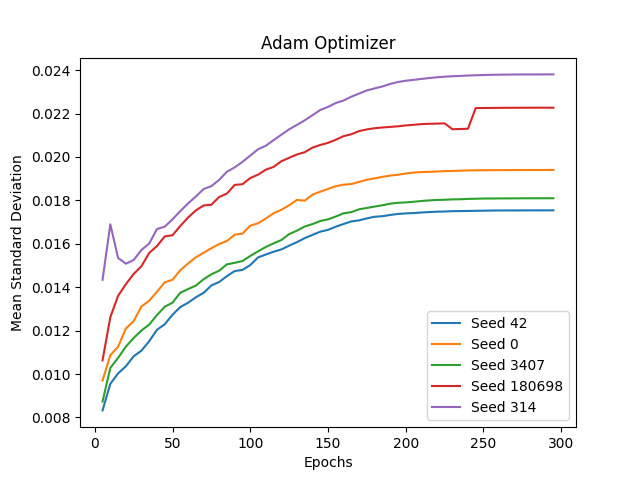
\includegraphics[width=\textwidth]{figures/cifar_adam_curves_std.png}
        \caption{CIFAR-10 Variances for ADAM Optimizer}
        \label{fig:cifar10_adam}
      \end{subfigure}
      \hfill
      \begin{subfigure}[b]{0.45\textwidth}
        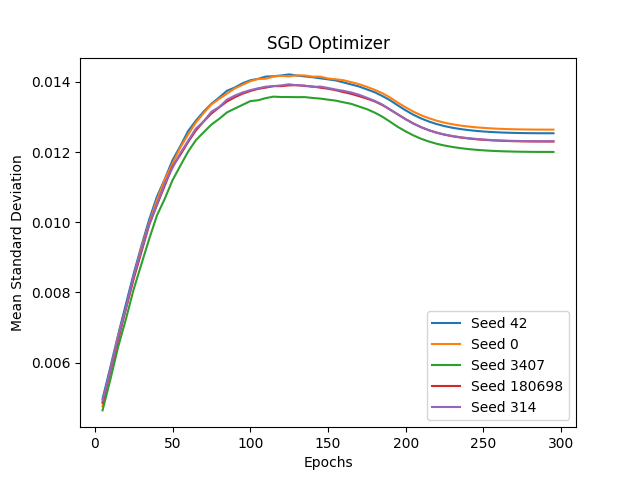
\includegraphics[width=\textwidth]{figures/cifar_sgd_curves_std.png}
        \caption{CIFAR-10 Variances for SGD Optimizer}
        \label{fig:cifar10_sgd}
      \end{subfigure}
      
      % CBIS-DDSM Row
      \begin{subfigure}[b]{0.45\textwidth}
        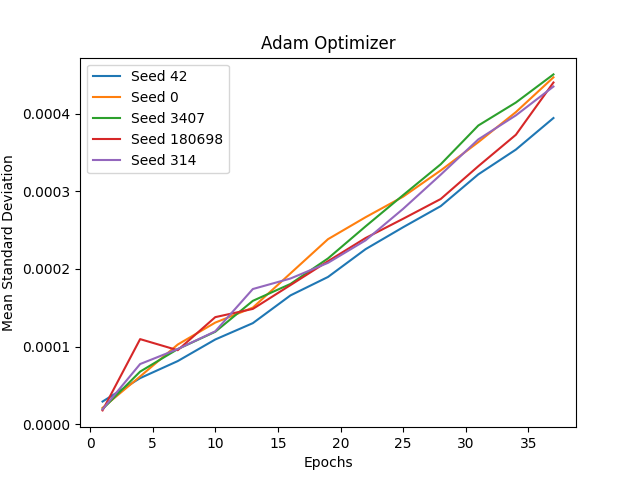
\includegraphics[width=\textwidth]{figures/mammo_adam_curvers_std.png}
        \caption{CBIS-DDSM Variances for ADAM Optimizer}
        \label{fig:cbisddsm_adam}
      \end{subfigure}
      \hfill
      \begin{subfigure}[b]{0.45\textwidth}
        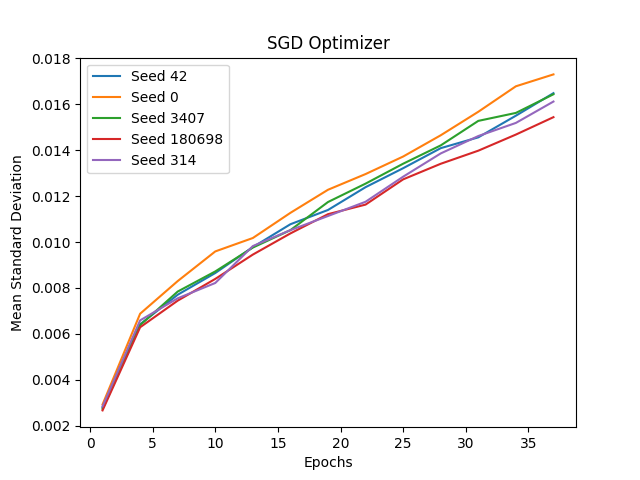
\includegraphics[width=\textwidth]{figures/mammo_sgd_curves_std.png}
        \caption{CBIS-DDSM Variances for SGD Optimizer}
        \label{fig:cbisddsm_sgd}
      \end{subfigure}
      
      % SDNET Row
      \begin{subfigure}[b]{0.45\textwidth}
        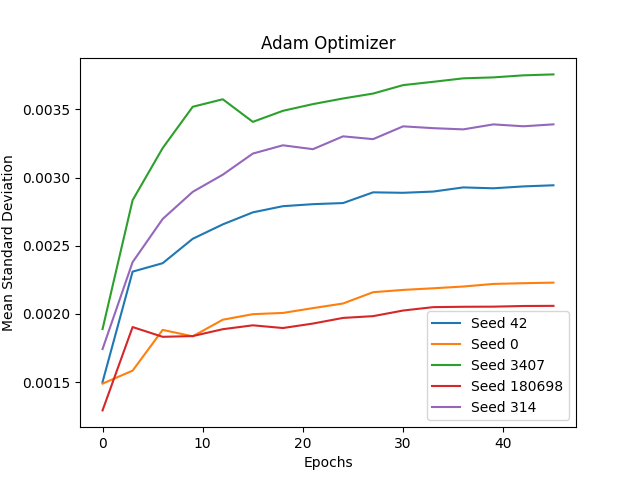
\includegraphics[width=\textwidth]{figures/crack_adam_curves_std.png}
        \caption{SDNET Variances for ADAM Optimizer}
        \label{fig:sdnet_adam}
      \end{subfigure}
      \hfill
      \begin{subfigure}[b]{0.45\textwidth}
        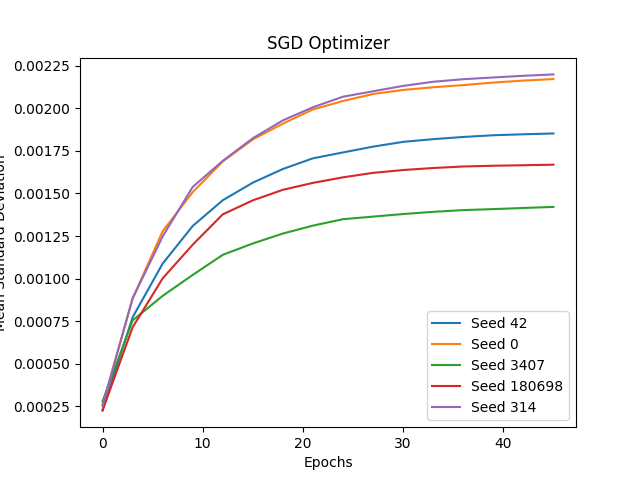
\includegraphics[width=\textwidth]{figures/crack_sgd_curves.png}
        \caption{SDNET Variances for SGD Optimizer}
        \label{fig:sdnet_sgd}
      \end{subfigure}
      
      \caption{Variance plots for different datasets and optimizers}
      \label{fig:variance_plots}
    \end{figure}

\clearpage    
By calculating the standart deviation, we aim to see how diverse is the particular weight index comparing the other identical runs that have inherent cuda randomness.
At a specific epoch, we take the weights from the five non-deterministic matrix and calculate the standart deviation componentwise. We end up with standart deviation matrix with the same dimensions.
Then first we take the mean in first direction then in second direction. As a result for each checkpoints we end up with one value that shows the mean standart variation in that specific epoch.
Below, we present the graphs for the three tasks.\\

In the figure \ref{fig:cifar10_adam}, mean standart deviations accros checkpoints are presentend. We observe
an increasing trend accross epochs. First standart variation values is calculated at fifth epochs so we have already weight updates and thus already far away from the initialization. But the reason that
it increases because we are fixing seed so in first steps weights are actually close to each other then with the CUDA randomness involved with each weight update it gets far away. Whenever the model converges and weights are not updated, we observe constant weights after approximately 200 epochs.
We also observe different seed values resulting in different variances. Seed values 314 and 180698 show less stable trends then the other and we observe some jumps during the training.\\

From the performance metrics we already observed that in CIFAR-10 dataset SGD optimizer shows more stable performance. Figure \ref{fig:cifar10_sgd} also supporst this claim as we see accros seed values similar variances. 
The curves are smoother than the ones with ADAM optimizer as well. Furthermore, unlike ADAM optimizer, with SGD optimizer we achieve decline in variances as the model converges then shows constand trend again.\\
Ultimately, we see lower variances than in the figure \ref{fig:cifar10_adam}\\

In mammography task which results shown in figures \ref{fig:cbisddsm_adam} and \ref{fig:cbisddsm_sgd}, some difficult situations arise and here we only have 40 epochs due to limitations. The model also does not show any concrete improvements after the 40. epoch. However, we see from the figures variances increase during training and we do not know whether they converges or not.
Important point here is that variance values, namely the range of variances are far less then CIFAR-10 dataset. We also see no distinct differences accros different seed values.\\

In the figures \ref{fig:sdnet_adam} and \ref{fig:sdnet_sgd}  we see the mean standart deviations accros epochs for concrete crack detection task for ADAM optimizer.
Unlike other two datasets, seed configurations seems to be more sensitive to the variances. From the start we see upward trend but variances tends to not drastically change after 15.epoch.
We observe the highest variance overall in seed as 3407.\\

For the SGD optimizer, stability seems to be better than the ADAM. Interestingly, we saw in the previous figures related to this task that ADAM optimizer was more stable.
The range of variances and the difference between seed values are also less than ADAM optimizer.
% (fix the labels on the y-axis)\\



\subsection{Similarities}

Apart from the variances, similarities between the weights in the last layer can be calculated. These similarity values can help
identify how much the matrices got far away from each other. Detailed information on how similarities calculated can be found in the previous section.\\

In the below figures that shows these similarities accros datasets and optimizers, we show minimum and mean similarities. While the mean similarities shows us the general trend. 
Minimum similarity indicates the extremum points of two runs that have inherent CUDA execution randomness. We understand from the minimal similarity the maximum potential that this randomness could have.
In the figures, 1 means the matrixes were identical and 0 means their subspace vectors completely orthogonal.
\clearpage

\begin{figure}[h!]
      \centering
      \begin{subfigure}[b]{0.3\textwidth}
        \includegraphics[width=\textwidth]{figures/cifar_similarities_Adam_V2.png}
        \caption{CIFAR-10 Similarities}
        \label{fig:cifar10_adam}
      \end{subfigure}
      \hfill % this will create horizontal space between figures
      \begin{subfigure}[b]{0.3\textwidth}
        \includegraphics[width=\textwidth]{figures/mammo_similarities_Adam_V2.png}
        \caption{CBIS-DDSM Similarities}
        \label{fig:cbisddsm_adam}
      \end{subfigure}
      \hfill
      \begin{subfigure}[b]{0.3\textwidth}
        \includegraphics[width=\textwidth]{figures/crack_similarities_Adam_V2.png}
        \caption{SDNET Similarities}
        \label{fig:sdnet_adam}
      \end{subfigure}
      \caption{Similarities in the Last Layer for ADAM Optimizer}
      \label{fig:similarities_adam}
\end{figure}


Figure \ref{fig:similarities_adam} illustrates the last layer similarities for the ADAM optimizer across various datasets. For the \textbf{CIFAR-10} dataset, the similarities commence at higher values, suggesting that the weights are initially alike. As training advances, these similarities predominantly decrease, indicating a divergence in weights. However, there's a subtle uptrend in the latter epochs, suggesting a resurgence in weight similarity. This trend is more pronounced in CIFAR-10 compared to other datasets. In the \textbf{CBIS-DDSM} dataset, there is a consistent decline in similarity. This consistent reduction may be attributed to the effects of finetuning from ImageNet-initialized weights rather than training from scratch. For the \textbf{SDNET} dataset, a pronounced initial drop is observed, indicating a swift divergence of weights. Yet, the similarities in subsequent epochs decline more gradually, hinting at a plateau in weight divergence. \\

Figure \ref{fig:similarities_sgd} represents the SGD optimizer's performance. The \textbf{CIFAR-10} dataset showcases stability in weight similarities throughout its training. There's a mild upward trend post-convergence, and notably, the weights remain more similar throughout this training phase compared to their ADAM optimizer counterparts. For the \textbf{CBIS-DDSM} dataset, the similarity curve is relatively stable, with a deceleration in the reduction of similarity as training matures. This trend hints at the potential stabilization of weights if training were to be extended. The \textbf{SDNET} dataset, although reminiscent of the ADAM optimizer in trend, is discernibly smoother. As training progresses, the weights tend to maintain their similarity, diverging less than with the ADAM optimizer.\\


\clearpage

\begin{figure}[h!]
      \centering
      \begin{subfigure}[b]{0.3\textwidth}
        \includegraphics[width=\textwidth]{figures/cifar_similarities_SGD_V2.png}
        \caption{CIFAR-10 Similarities}
        \label{fig:cifar10_sgd}
      \end{subfigure}
      \hfill % this will create horizontal space between figures
      \begin{subfigure}[b]{0.3\textwidth}
        \includegraphics[width=\textwidth]{figures/mammo_similarities_SGD_V2.png}
        \caption{CBIS-DDSM Similarities}
        \label{fig:cbisddsm_sgd}
      \end{subfigure}
      \hfill
      \begin{subfigure}[b]{0.3\textwidth}
        \includegraphics[width=\textwidth]{figures/crack_similarities_SGD_V2.png}
        \caption{SDNET Similarities}
        \label{fig:sdnet_sgd}
      \end{subfigure}
      \caption{Similarities in the Last Layer for SGD Optimizer}
      \label{fig:similarities_sgd}
\end{figure}


\clearpage




\section{Statistical Tests} 

Statistical tests are essential tools in research, enabling scientists to infer or deduce properties about a population based on a sample. These tests provide a framework to make decisions or judgments about parameters or datasets by considering the likelihood that an observed outcome would happen due to chance alone.

\subsection{T-Test with Population Mean} 
The t-test is a statistical procedure used to determine whether there is a significant difference between the means of two groups. In this specific application, the t-test is being used to compare the performance values from non-deterministic runs with a known population mean.
The idea behind using the deterministic run as the population mean is grounded in the assumption that the deterministic run will consistently produce the same results regardless of the number of times it is executed. This makes it an appropriate stand-in for the "true" population mean.

Given this setup, the t-test is framed as:

\begin{enumerate}
    \item \textbf{Null Hypothesis ($H_0$)}: There is no significant difference between the performance values of the non-deterministic runs and the deterministic run (population mean).
    \item \textbf{Alternative Hypothesis ($H_1$)}: There is a significant difference between the performance values of the non-deterministic runs and the deterministic run.
\end{enumerate}

The resultant p-value from the t-test signifies the probability of observing the given data (or more extreme data) if the null hypothesis holds true. Conventionally, a threshold of $p < 0.05$ is used to denote statistical significance. A p-value below this threshold implies that the observed data is inconsistent with the null hypothesis, leading to its rejection in favor of the alternative hypothesis.

\begin{table}[h!]
      \centering
      \caption{Statistical Test Results for all datasets}
      \label{tab:stat_results}
      \begin{tabular}{|l|r|l|c|c|c|}
      \toprule
      \textbf{Seed} & \textbf{Optimizer} & \textbf{CIFAR-10 P-Value} & \textbf{CBIS-DDSM P-Value} & \textbf{SDNET P-Value} \\
      \hline
       0 & ADAM & \cellcolor{myred} 0.008406 & \cellcolor{myred} 0.000976 & \cellcolor{myred} 0.000889 \\
      \hline
       0 & SGD & \cellcolor{myyellow} 0.069109 & \cellcolor{mygreen} 0.218819 & \cellcolor{mygreen} 0.429838 \\
      \hline
      180698 & ADAM & \cellcolor{myred} 0.004008 & \cellcolor{myred} 0.033590 & \cellcolor{myred} 0.013022 \\
      \hline
       180698 & SGD & \cellcolor{myyellow} 0.063953 & \cellcolor{myred} 0.026436 & \cellcolor{mygreen} 0.147029 \\
      \hline
       314 & ADAM & \cellcolor{mygreen} 0.975627 & \cellcolor{myred} 0.003490 & \cellcolor{mygreen} 0.463445 \\
      \hline
       314 & SGD & \cellcolor{mygreen} 0.295095 & \cellcolor{mygreen} 0.522252 & \cellcolor{myred} 0.001812 \\
      \hline
       3407 & ADAM & \cellcolor{mygreen} 0.373808 & \cellcolor{myred} 0.046387 & \cellcolor{myyellow} 0.088054 \\
      \hline
       3407 & SGD & \cellcolor{myyellow} 0.069981 & \cellcolor{mygreen} 0.230912 & \cellcolor{mygreen} 0.543679 \\
      \hline
       42 & ADAM & \cellcolor{mygreen} 0.215843 & \cellcolor{myred} 0.005721 & \cellcolor{mygreen} 0.102999 \\
      \hline
       42 & SGD & \cellcolor{mygreen} 0.326455 & \cellcolor{mygreen} 0.516847 & \cellcolor{myred} 0.006795 \\
      \hline
      \end{tabular}
\end{table}


Examining the table, it's evident that different configurations yield varying levels of statistical significance across the datasets. We'll break down the observations dataset by dataset:


\begin{enumerate}
      \item \textbf{CIFAR-10 Dataset}:
      \begin{itemize}
          \item Of the 10 configurations, a mere 2 employing the ADAM optimizer manifest statistically significant results, as evinced by their p-values being beneath 0.05.
          \item A majority of the configurations, notably those using the SGD optimizer, seem congruent with the deterministic run, implying the reliability of results from these configurations.
      \end{itemize}
      
      \item \textbf{CBIS-DDSM Dataset}:
      \begin{itemize}
          \item All configurations that harness the ADAM optimizer have been marked as statistically significant, suggesting potential unreliability of results from these configurations.
          \item A solitary configuration with the SGD optimizer points towards statistical significance.
          \item This insinuates that while the SGD optimizer is predominantly consistent with the deterministic run for this dataset, configurations with the ADAM optimizer might necessitate additional runs or enhanced reproducibility protocols.
      \end{itemize}
      
      \item \textbf{SDNET Dataset}:
      \begin{itemize}
          \item Both the ADAM and SGD optimizers have a pair of configurations each that are flagged as statistically significant.
          \item The remaining configurations seem to be in harmony with the deterministic run, indicating their reliability for the concrete crack detection task.
      \end{itemize}
  \end{enumerate}

In summary, the results highlight the importance of reproducibility and consistency in experiments, especially when working with non-deterministic configurations. The choice of optimizer, as well as other experimental parameters, can significantly influence the reliability of results. It's crucial to consider these factors and conduct appropriate statistical tests to ensure the robustness of findings.

\subsection{ANOVA and Kruskal-Wallis Tests}

In the T-Test with population mean we investigated the the statistical significance for
each configurations. But we can direct our focus on the optimizer sensitivity and use the ANOVA (Analysis of Variance) and Kruskal-Wallis tests. These tests stand out as important tools. Both are designed to determine if there are any statistically significant differences between the means of three or more independent (unrelated) groups. ANOVA, being parametric, is apt for data that is normally distributed. On the other hand, the Kruskal-Wallis test, a non-parametric method, comes into play when the assumption of normality isn't met.\\

For our study's context, these tests offer invaluable insights. They help discern performance differences between various optimizers across multiple datasets. By comparing the means of different configurations for each optimizer, we can determine if an optimizer consistently outperforms others or if the observed differences are mere products of random chance.\\

The results of both tests for the optimizers ADAM and SGD, evaluated across three datasets: Cifar-10, Mammography, and Crack Detection, are presented in Table~\ref{tab:anova_kruskal_results}. The F-Value (for ANOVA) and the test statistic (for Kruskal-Wallis) provide the test's outcome, while the P-Value is our key to determining the significance of these results.\\

\begin{table}[h!]
      \centering
      \caption{ANOVA and Kruskal-Wallis Test Results for Optimizers across Datasets}
      \label{tab:anova_kruskal_results}
      \begin{tabularx}{\textwidth}{
            l
            l
            S[table-format=2.5]@{\hspace{0.65em}}
            S[table-format=1.4]
            S[table-format=2.2]@{\hspace{0.65em}}
            S[table-format=1.4]
            S[table-format=1.2]@{\hspace{0.65em}}
            S[table-format=1.3]
      }
            \toprule
            \multirow{2}{*}{Test} & \multirow{2}{*}{Optimizer} & \multicolumn{2}{c}{Cifar-10} & \multicolumn{2}{c}{Mammography} & \multicolumn{2}{c}{Crack Detection} \\
            \cmidrule(lr){3-4} \cmidrule(lr){5-6} \cmidrule(lr){7-8}
             & & {F-Value} & {P-Value} & {F-Value} & {P-Value} & {F-Value} & {P-Value} \\
            \midrule
            ANOVA          & ADAM & 3.24    & 0.027  &  9.56 & 0.0001 & 2.11 & 0.117 \\
            Kruskal-Wallis & ADAM & 7.73    & 0.101  & 16.78 & 0.0021 & 7.28 & 0.121 \\
            ANOVA          & SGD  & 0.63    & 0.6438 &  0.53 & 0.7086 & 3.43 & 0.026 \\
            Kruskal-Wallis & SGD  & 2.06    & 0.7246 &  2.36 & 0.6693 & 8.66 & 0.069 \\
            \bottomrule
      \end{tabularx}
\end{table}
      
\textbf{ADAM Optimizer:} For the Cifar-10 dataset, the ANOVA test's P-Value stands at 0.027, hinting at significant differences between the means of the groups. However, the Kruskal-Wallis test suggests no significant difference with a P-Value of 0.101. For the Mammography dataset, both tests indicate significant differences between the groups, with P-Values of 0.0001 (ANOVA) and 0.0021 (Kruskal-Wallis). On the Crack Detection dataset, neither test shows a significant difference with P-Values of 0.117 (ANOVA) and 0.121 (Kruskal-Wallis).\\

\textbf{SGD Optimizer:} For the Cifar-10 dataset, both tests converge on the same conclusion: no significant difference in the means of the groups with P-Values of 0.6438 (ANOVA) and 0.7246 (Kruskal-Wallis). Similarly, for the Mammography dataset, both tests indicate no significant difference. However, for the Crack Detection dataset, ANOVA suggests a significant difference with a P-Value of 0.026, while the Kruskal-Wallis test doesn't corroborate this, presenting a P-Value of 0.069.\\

\clearpage

